

\tikzset{every picture/.style={line width=0.75pt}} %set default line width to 0.75pt        

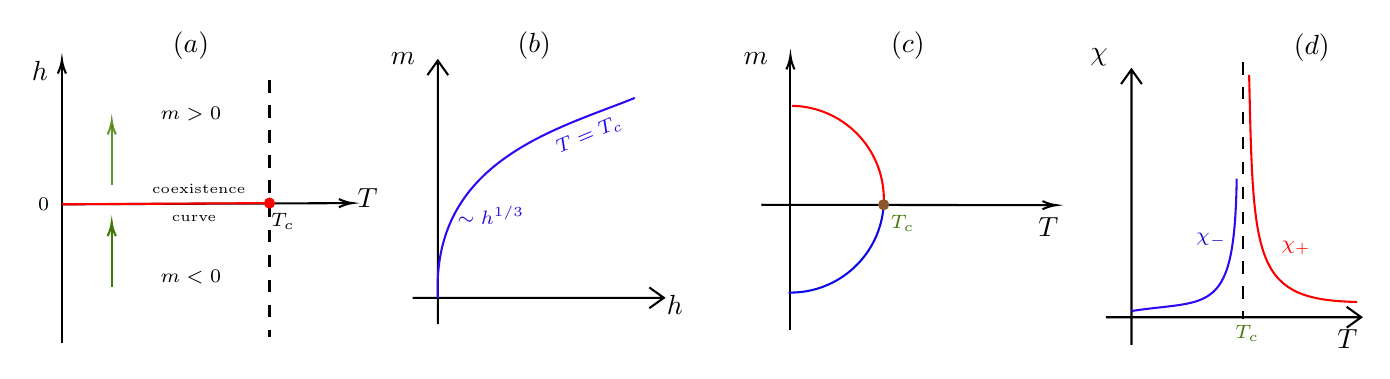
\begin{tikzpicture}[x=0.75pt,y=0.75pt,yscale=-1,xscale=1]
%uncomment if require: \path (0,300); %set diagram left start at 0, and has height of 300

%Straight Lines [id:da6405013566248435] 
\draw  [dash pattern={on 4.5pt off 4.5pt}]  (123,50.33) -- (123,173.92) ;
%Straight Lines [id:da1771009790917556] 
\draw    (23,110) -- (161,109.43) ;
\draw [shift={(163,109.42)}, rotate = 179.76] [color={rgb, 255:red, 0; green, 0; blue, 0 }  ][line width=0.75]    (6.56,-1.97) .. controls (4.17,-0.84) and (1.99,-0.18) .. (0,0) .. controls (1.99,0.18) and (4.17,0.84) .. (6.56,1.97)   ;
%Straight Lines [id:da04196864778525011] 
\draw    (23,177) -- (23,42.42) ;
\draw [shift={(23,40.42)}, rotate = 90] [color={rgb, 255:red, 0; green, 0; blue, 0 }  ][line width=0.75]    (6.56,-1.97) .. controls (4.17,-0.84) and (1.99,-0.18) .. (0,0) .. controls (1.99,0.18) and (4.17,0.84) .. (6.56,1.97)   ;
%Straight Lines [id:da01493162060557951] 
\draw [color={rgb, 255:red, 255; green, 0; blue, 0 }  ,draw opacity=1 ]   (23,110) -- (122,109.42) ;
%Shape: Circle [id:dp867729571200196] 
\draw  [draw opacity=0][fill={rgb, 255:red, 255; green, 0; blue, 0 }  ,fill opacity=1 ] (120.29,109.42) .. controls (120.29,107.92) and (121.5,106.71) .. (123,106.71) .. controls (124.5,106.71) and (125.71,107.92) .. (125.71,109.42) .. controls (125.71,110.91) and (124.5,112.13) .. (123,112.13) .. controls (121.5,112.13) and (120.29,110.91) .. (120.29,109.42) -- cycle ;
%Shape: Axis 2D [id:dp17193896756207128] 
\draw  (192,155.05) -- (313,155.05)(204.1,40.75) -- (204.1,167.75) (306,150.05) -- (313,155.05) -- (306,160.05) (199.1,47.75) -- (204.1,40.75) -- (209.1,47.75)  ;
%Curve Lines [id:da7690846074551628] 
\draw [color={rgb, 255:red, 47; green, 9; blue, 243 }  ,draw opacity=1 ]   (204.1,155.05) .. controls (201,88.75) and (262,73.75) .. (299,58.75) ;
%Straight Lines [id:da7792025510369985] 
\draw [color={rgb, 255:red, 65; green, 117; blue, 5 }  ,draw opacity=1 ]   (47,149.75) -- (47,120.75) ;
\draw [shift={(47,118.75)}, rotate = 90] [color={rgb, 255:red, 65; green, 117; blue, 5 }  ,draw opacity=1 ][line width=0.75]    (6.56,-1.97) .. controls (4.17,-0.84) and (1.99,-0.18) .. (0,0) .. controls (1.99,0.18) and (4.17,0.84) .. (6.56,1.97)   ;
%Straight Lines [id:da9412226479737181] 
\draw [color={rgb, 255:red, 72; green, 129; blue, 6 }  ,draw opacity=0.84 ]   (47,100.75) -- (47,71.75) ;
\draw [shift={(47,69.75)}, rotate = 90] [color={rgb, 255:red, 72; green, 129; blue, 6 }  ,draw opacity=0.84 ][line width=0.75]    (6.56,-1.97) .. controls (4.17,-0.84) and (1.99,-0.18) .. (0,0) .. controls (1.99,0.18) and (4.17,0.84) .. (6.56,1.97)   ;
%Straight Lines [id:da022225285664967287] 
\draw    (360,110.23) -- (500,110.41) ;
\draw [shift={(502,110.42)}, rotate = 180.07] [color={rgb, 255:red, 0; green, 0; blue, 0 }  ][line width=0.75]    (6.56,-1.97) .. controls (4.17,-0.84) and (1.99,-0.18) .. (0,0) .. controls (1.99,0.18) and (4.17,0.84) .. (6.56,1.97)   ;
%Straight Lines [id:da5955194158187582] 
\draw    (374,170.65) -- (374,40.43) ;
\draw [shift={(374,38.43)}, rotate = 90] [color={rgb, 255:red, 0; green, 0; blue, 0 }  ][line width=0.75]    (6.56,-1.97) .. controls (4.17,-0.84) and (1.99,-0.18) .. (0,0) .. controls (1.99,0.18) and (4.17,0.84) .. (6.56,1.97)   ;
%Shape: Arc [id:dp3444542517243655] 
\draw  [draw opacity=0] (374.79,62.55) .. controls (399.28,62.97) and (419,82.95) .. (419,107.54) .. controls (419,108.53) and (418.97,109.51) .. (418.91,110.48) -- (374,107.54) -- cycle ; \draw  [color={rgb, 255:red, 255; green, 0; blue, 0 }  ,draw opacity=1 ] (374.79,62.55) .. controls (399.28,62.97) and (419,82.95) .. (419,107.54) .. controls (419,108.53) and (418.97,109.51) .. (418.91,110.48) ;  
%Shape: Arc [id:dp7404940238529929] 
\draw  [draw opacity=0] (418.9,110.49) .. controls (417.38,133.97) and (397.86,152.54) .. (374,152.54) .. controls (373.71,152.54) and (373.41,152.54) .. (373.12,152.53) -- (374,107.54) -- cycle ; \draw  [color={rgb, 255:red, 11; green, 7; blue, 233 }  ,draw opacity=1 ] (418.9,110.49) .. controls (417.38,133.97) and (397.86,152.54) .. (374,152.54) .. controls (373.71,152.54) and (373.41,152.54) .. (373.12,152.53) ;  
%Shape: Circle [id:dp5353821681280311] 
\draw  [draw opacity=0][fill={rgb, 255:red, 139; green, 87; blue, 42 }  ,fill opacity=0.99 ] (416.2,110.19) .. controls (416.2,108.69) and (417.41,107.48) .. (418.91,107.48) .. controls (420.4,107.48) and (421.61,108.69) .. (421.61,110.19) .. controls (421.61,111.68) and (420.4,112.89) .. (418.91,112.89) .. controls (417.41,112.89) and (416.2,111.68) .. (416.2,110.19) -- cycle ;
%Shape: Axis 2D [id:dp6659037135296868] 
\draw  (526,164.41) -- (649,164.41)(538.3,45.05) -- (538.3,177.67) (642,159.41) -- (649,164.41) -- (642,169.41) (533.3,52.05) -- (538.3,45.05) -- (543.3,52.05)  ;
%Straight Lines [id:da7336090114018968] 
\draw  [dash pattern={on 4.5pt off 4.5pt}]  (592,41.48) -- (592,165.08) ;
%Curve Lines [id:da16499067493517872] 
\draw [color={rgb, 255:red, 47; green, 9; blue, 243 }  ,draw opacity=1 ]   (538.3,161.41) .. controls (576,155.62) and (588,164.62) .. (589,97.62) ;
%Curve Lines [id:da09998300021371642] 
\draw [color={rgb, 255:red, 252; green, 0; blue, 0 }  ,draw opacity=1 ]   (647,157.05) .. controls (597,156.05) and (597,138.05) .. (595,47.62) ;

% Text Node
\draw (180,35.4) node [anchor=north west][inner sep=0.75pt]    {$m$};
% Text Node
\draw (313,152.4) node [anchor=north west][inner sep=0.75pt]    {$h$};
% Text Node
\draw (258.24,78.85) node [anchor=north west][inner sep=0.75pt]  [font=\scriptsize,color={rgb, 255:red, 31; green, 7; blue, 243 }  ,opacity=1 ,rotate=-337.1]  {$T=T_{c}$};
% Text Node
\draw (212,109.4) node [anchor=north west][inner sep=0.75pt]  [font=\scriptsize,color={rgb, 255:red, 53; green, 11; blue, 218 }  ,opacity=1 ]  {$\sim h^{1/3}$};
% Text Node
\draw (7,39.4) node [anchor=north west][inner sep=0.75pt]    {$h$};
% Text Node
\draw (164,100.82) node [anchor=north west][inner sep=0.75pt]    {$T$};
% Text Node
\draw (122.29,112.82) node [anchor=north west][inner sep=0.75pt]  [font=\scriptsize]  {$T_{c}$};
% Text Node
\draw (10,105.4) node [anchor=north west][inner sep=0.75pt]  [font=\scriptsize]  {$0$};
% Text Node
\draw (75,25.4) node [anchor=north west][inner sep=0.75pt]    {$( a)$};
% Text Node
\draw (241,25.4) node [anchor=north west][inner sep=0.75pt]    {$( b)$};
% Text Node
\draw (350,35.4) node [anchor=north west][inner sep=0.75pt]    {$m$};
% Text Node
\draw (420.9,113.89) node [anchor=north west][inner sep=0.75pt]  [font=\scriptsize,color={rgb, 255:red, 65; green, 117; blue, 5 }  ,opacity=1 ]  {$T_{c}$};
% Text Node
\draw (421,25.4) node [anchor=north west][inner sep=0.75pt]    {$( c)$};
% Text Node
\draw (492,114.82) node [anchor=north west][inner sep=0.75pt]    {$T$};
% Text Node
\draw (609,126.4) node [anchor=north west][inner sep=0.75pt]  [font=\scriptsize,color={rgb, 255:red, 255; green, 10; blue, 0 }  ,opacity=1 ]  {$\chi _{+}$};
% Text Node
\draw (568,122.4) node [anchor=north west][inner sep=0.75pt]  [font=\scriptsize,color={rgb, 255:red, 22; green, 11; blue, 206 }  ,opacity=1 ]  {$\chi _{-}$};
% Text Node
\draw (586.9,166.89) node [anchor=north west][inner sep=0.75pt]  [font=\scriptsize,color={rgb, 255:red, 65; green, 117; blue, 5 }  ,opacity=1 ]  {$T_{c}$};
% Text Node
\draw (636,168.82) node [anchor=north west][inner sep=0.75pt]    {$T$};
% Text Node
\draw (517,33.4) node [anchor=north west][inner sep=0.75pt]    {$\chi $};
% Text Node
\draw (615,26.4) node [anchor=north west][inner sep=0.75pt]    {$( d)$};
% Text Node
\draw (65,99) node [anchor=north west][inner sep=0.75pt]  [font=\tiny] [align=left] {coexistence};
% Text Node
\draw (74.5,113.71) node [anchor=north west][inner sep=0.75pt]  [font=\tiny] [align=left] {curve};
% Text Node
\draw (69,140.4) node [anchor=north west][inner sep=0.75pt]  [font=\scriptsize]  {$m< 0$};
% Text Node
\draw (69,61.4) node [anchor=north west][inner sep=0.75pt]  [font=\scriptsize]  {$m >0$};


\end{tikzpicture}
